%
% k-gravitatzion.tex
%
% (c) 2017 Prof Dr Andreas Müller, Hochschule Rapperswil
%
\section{Gravitation%
\label{skript:kruemmusng:sectipn:gravitation}}
Albert Einstein hat erkannt, dass die Wirkung der Gravitation 
durch die Krümmung des Raumes beschrieben werden muss.
\index{Einstein, Albert}

%\subsection{Speziellue Relativitätstheorie}
%Im neunzehnten Jahrhundert hat James Clark Maxwell die Theorien
%über Elektriztität und Magnetismus zu einer einheitlichen Theorie
%der Elektrodynamik zusammengefasst.
%\index{Maxwell, James Clark}
%\index{Elektrodynamik}
%Diese Theorie ist die Grundlage aller Phänomene, mit denen sich
%ein Elektroingenieur täglich herumschlägt.
%Sie hat jedoch eine seltsame Eigenschaft, die schon sehr früh
%aufgefallen ist.
%Die Formeln der Mechanik von Galilei und Newton nicht ändern,
%wenn man eine Koordinatentransformation der Form
%\begin{equation}
%\begin{aligned}
%t'&=t\\
%x'&=x+vt
%\end{aligned}
%\label{skript:kruemmung:galileitransformation}
%\end{equation}
%\index{Galiei-Transformation}
%durchführt.
%Diese Koordinatentransformation entspricht einer gleichförmigen
%Bewegung des $(t',x')$-Koordinatensystems gegenüber dem 
%$(t,x)$-Koordinatensystem.
%Sie wird auch Galilei-Transformation genannt und wiederspiegelt die
%Erfahrungstatsache, dass es in einem abfahrenden Zug schwierig ist
%zu entscheiden, ob sich nun der Zug oder der Bahnhof in Bewegung setzt.
%
%Die Gleichungen der Elektrodynamik verändern sich jedoch.
%Es stellte sich daher die Frage, ob die Gleichungen der Elektrodynamik
%nur einen Teilaspekt der Realität darstellen, oder ob die Gleichungen
%der Mechanik nur eine Näherung sind, die für Geschwindigkeiten nahe
%der Lichtgeschwindigkeiten nicht mehr zulässig sein würden.
%Im letzten Fall wäre die
%Galilei-Transformation~\eqref{skript:kruemmung:galileitransformation}
%für solche Geschwidigkeiten auch nur eine Näherung, die durch
%eine exaktere Formel ersetzt werden müsste, mit weitreichenden
%Folgen für die Mechanik bei sehr hohen Geschwindigkeiten.
%
%Es hat sich herausgestellt, dass tatsächlich die klassische Mechanik
%angepasst werden muss.
%Einstein hat diesen Schritt 1905 in seiner speziellen Relativitätstheorie
%vollzogen.
%Ziel dieses Abschnittes ist zu zeigen, welche Auswirkungen seine
%Erkenntnis auf die Mechanik aber auch auf unser Weltbild hat.
%
%\subsubsection{Lichtkegel}
%Die Elektrodynamik sagt die Ausbreitungsgeschwindigkeit von
%elektromagnetishen Wellen voraus.
%Stellt man sich vor, dass elektromagnetische Wellen von einem
%Medium geleitet werden, das man Äther nannte, dann müsste die
%Geschwindigkeit von der Bewegung des Beobachters relativ zu
%diesem Äther abhängen.
%In hochgenauen Experimenten konnten Michelson und Morley und später
%viele andere keine solche Abhängigkeit feststellen.
%Dies steht zwar in Einklang mit der Theorie der Elektrodynamik,
%wiederspricht der Galilei-Transformation, welche eine Veränderung
%der Ausbreitungsgeschwindigkeit um $v$ vorhersagen würde.
%
%Einstein hat die experimentell sehr gut bestätigte Konstanz der
%Lichtgeschwindigkeit daher als Ausgangspunkt seiner Theorie genommen.
%Entscheidend für die Physik ist, ob zwei Punkte sich mit elektromagnetischen
%Wellen beeinflussen können.
%Es ist daher nicht mehr ausreichend, nur Punkte miteinander zu vergleichen,
%es muss auch immer die Zeit berücksichtigt werden, zu der sie verglichen
%werden.
%Raum und Zeit verschmelzen so zu einem einzigen vierdimensionalen
%Kontinuum mit den Koordinaten $(t,x,y,z)$, welche wir die Raumzeit
%nennen.
%Quadrupel $(t,x,y,z)$ heissen auch {\em Ereignisse}.
%\index{Ereignis}
%
%\begin{figure}
%\centering
%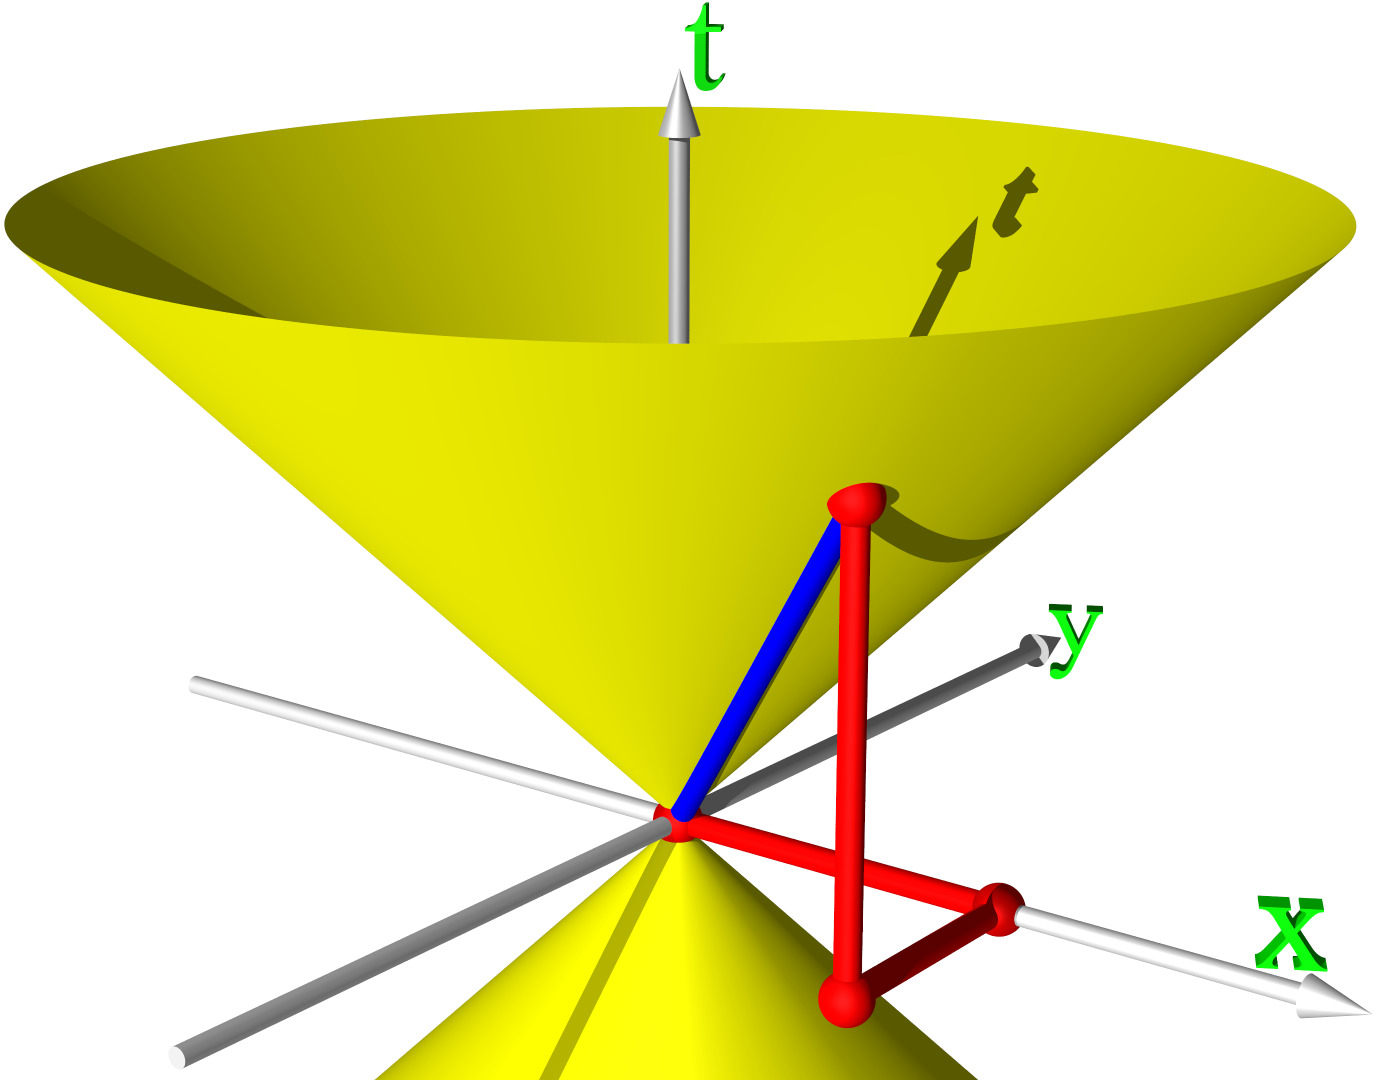
\includegraphics[width=\hsize]{chapters/3d/lichtkegel.jpg}
%\caption{Lichtkegel ausgehend vom Nullpunkt zur Zeit $t=0$.
%Alle Punkte innerhalb des Kegels mit $t>0$ liegen in der Zukunft des
%Beobachters im Nullpunkt, solche mit $t<0$ in seiner Vergangenheit.
%Punkte ausserhalb des Kegels können vom Nullpunkt aus nicht
%beeinflusst werden.
%Nur Punkte innerhalb des Kegels mit $t<0$ können Einfluss haben
%auf den Nullpunkt.
%\label{skript:kruemmung:fig:lichtkegel}}
%\end{figure}
%
%\subsubsection{Lorenztransformation}
%\subsubsection{Energie und Impuls}
%
%
% k-speziell.tex -- Spezielle Relativitätstheorie
%
% (c) 2017 Prof Dr Andreas Müller, Hochschule Rapperswil
%

\section{Spezielle Relativitätstheorie}
\rhead{Spezielle Relativitätstheorie}
Im neunzehnten Jahrhundert hat James Clark Maxwell die Theorien
über Elektriztität und Magnetismus zu einer einheitlichen Theorie
der Elektrodynamik zusammengefasst.
\index{Maxwell, James Clark}
\index{Elektrodynamik}
Diese Theorie ist die Grundlage aller Phänomene, mit denen sich
ein Elektroingenieur täglich herumschlägt.
Sie hat jedoch eine seltsame Eigenschaft, die schon sehr früh
aufgefallen ist.
Die Formeln der Mechanik von Galilei und Newton nicht ändern,
wenn man eine Koordinatentransformation der Form
\begin{equation}
\begin{aligned}
t'&=t\\
x'&=x+vt
\end{aligned}
\label{skript:kruemmung:galileitransformation}
\end{equation}
\index{Galiei-Transformation}
durchführt.
Diese Koordinatentransformation entspricht einer gleichförmigen
Bewegung des $(t',x')$-Koordinatensystems gegenüber dem 
$(t,x)$-Koordinatensystem.
Sie wird auch Galilei-Transformation genannt und wiederspiegelt die
Erfahrungstatsache, dass es in einem abfahrenden Zug schwierig ist
zu entscheiden, ob sich nun der Zug oder der Bahnhof in Bewegung setzt.

Die Gleichungen der Elektrodynamik verändern sich jedoch.
Es stellte sich daher die Frage, ob die Gleichungen der Elektrodynamik
nur einen Teilaspekt der Realität darstellen, oder ob die Gleichungen
der Mechanik nur eine Näherung sind, die für Geschwindigkeiten nahe
der Lichtgeschwindigkeiten nicht mehr zulässig sein würden.
Im letzten Fall wäre die
Galilei-Transformation~\eqref{skript:kruemmung:galileitransformation}
für solche Geschwidigkeiten auch nur eine Näherung, die durch
eine exaktere Formel ersetzt werden müsste, mit weitreichenden
Folgen für die Mechanik bei sehr hohen Geschwindigkeiten.

Es hat sich herausgestellt, dass tatsächlich die klassische Mechanik
angepasst werden muss.
Einstein hat diesen Schritt 1905 in seiner speziellen Relativitätstheorie
vollzogen.
Ziel dieses Abschnittes ist zu zeigen, welche Auswirkungen seine
Erkenntnis auf die Mechanik aber auch auf unser Weltbild hat.

\subsection{Lichtkegel}
Die Elektrodynamik sagt die Ausbreitungsgeschwindigkeit von
elektromagnetishen Wellen voraus.
Stellt man sich vor, dass elektromagnetische Wellen von einem
Medium geleitet werden, das man Äther nannte, dann müsste die
Geschwindigkeit von der Bewegung des Beobachters relativ zu
diesem Äther abhängen.
In hochgenauen Experimenten konnten Michelson und Morley und später
viele andere keine solche Abhängigkeit feststellen.
Dies steht zwar in Einklang mit der Theorie der Elektrodynamik,
wiederspricht der Galilei-Transformation, welche eine Veränderung
der Ausbreitungsgeschwindigkeit um $v$ vorhersagen würde.

Einstein hat die experimentell sehr gut bestätigte Konstanz der
Lichtgeschwindigkeit daher als Ausgangspunkt seiner Theorie genommen.
Entscheidend für die Physik ist, ob zwei Punkte sich mit elektromagnetischen
Wellen beeinflussen können.
Es ist daher nicht mehr ausreichend, nur Punkte miteinander zu vergleichen,
es muss auch immer die Zeit berücksichtigt werden, zu der sie verglichen
werden.
Raum und Zeit verschmelzen so zu einem einzigen vierdimensionalen
Kontinuum mit den Koordinaten $(t,x,y,z)$, welche wir die Raumzeit
nennen.
Quadrupel $(t,x,y,z)$ heissen auch {\em Ereignisse}.
\index{Ereignis}
Zwei Ereignisse $(t_1,x_1,y_1,z_1)$ und $(t_2,x_2,y_2,z_2)$ können
kausal voneinander abhängen, wenn ein Lichtsignal sich vom einen Ereignis
zum anderen Ereignis ausbreiten kann.
Dazu ist notwendig, dass der ``Abstand''
\begin{equation}
s^2
=
-c^2(t_1-t_2)^2
+
\mathstrut
\underbrace{
(x_1-x_2)^2
+
(y_1-y_2)^2
+
(z_1-z_2)^2}_{\text{Raumabstand}}
\label{skript:kruemmung:raumzeitabstand}
\end{equation}
gleich $0$ ist.
Breitet sich die Wirkung langsamer als mit Lichtgeschwindigket aus,
wird die zeitliche Differenz noch grösser sein, und damit der
Ausdruck~\eqref{skript:kruemmung:raumzeitabstand} negativ ist.

\begin{figure}
\centering
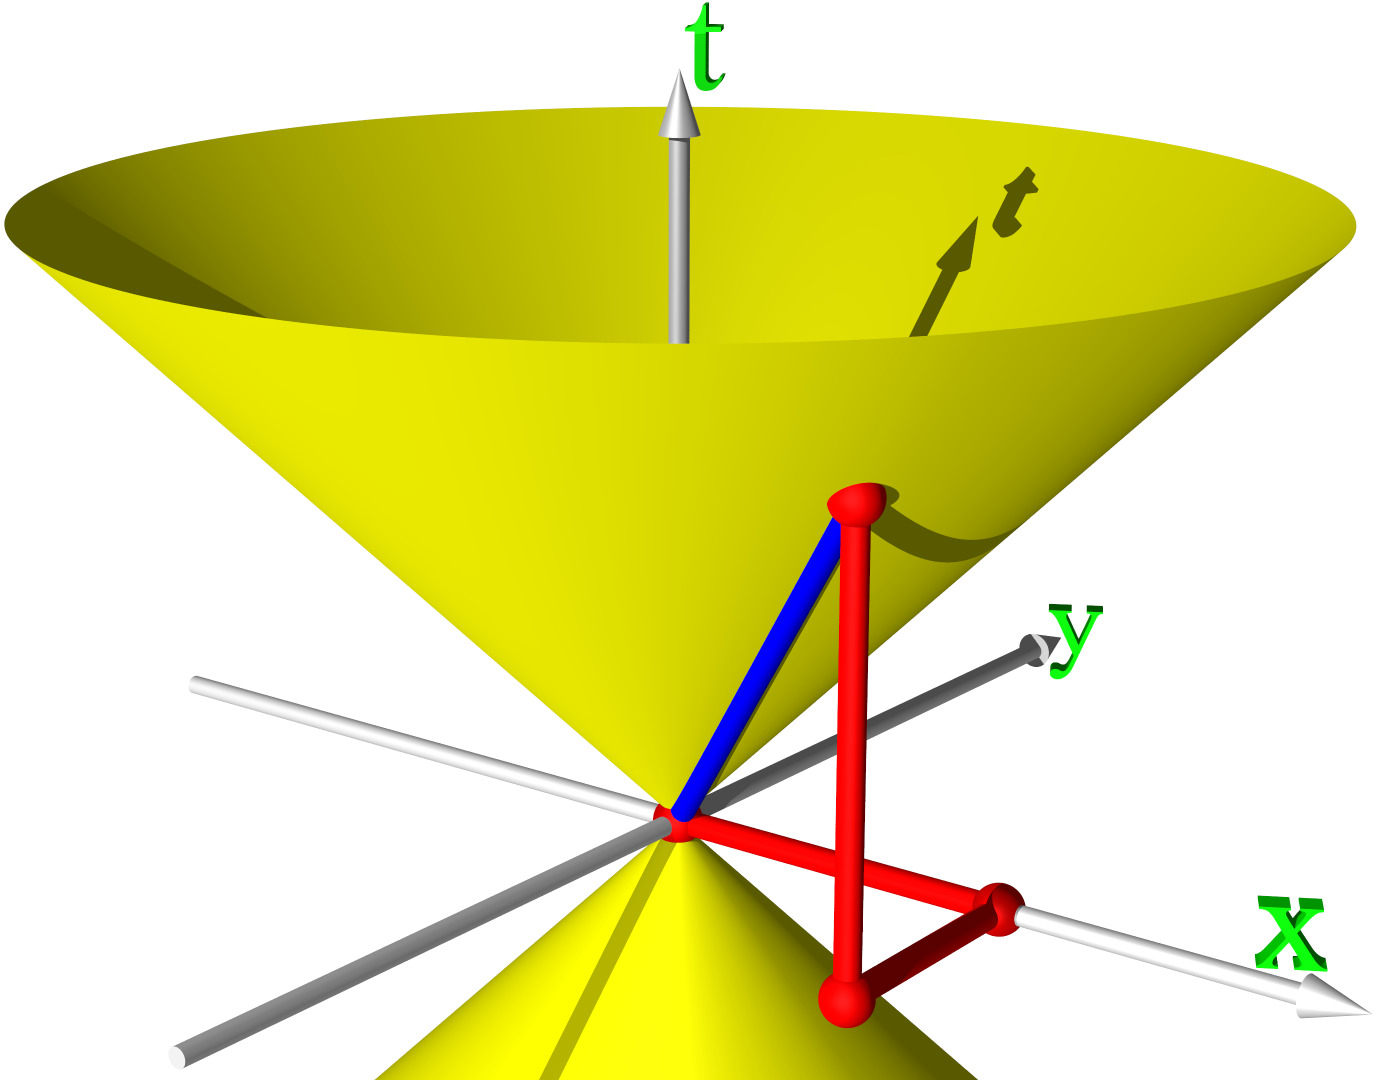
\includegraphics[width=\hsize]{chapters/3d/lichtkegel.jpg}
\caption{Lichtkegel ausgehend vom Nullpunkt zur Zeit $t=0$.
Alle Punkte innerhalb des Kegels mit $t>0$ liegen in der Zukunft des
Beobachters im Nullpunkt, solche mit $t<0$ in seiner Vergangenheit.
Punkte ausserhalb des Kegels können vom Nullpunkt aus nicht
beeinflusst werden.
Nur Punkte innerhalb des Kegels mit $t<0$ können Einfluss haben
auf den Nullpunkt.
\label{skript:kruemmung:fig:lichtkegel}}
\end{figure}

Das Vorzeichen des Ausdrucks~\eqref{skript:kruemmung:raumzeitabstand}
beschreibt also, ob zwei Ereignisse sich gegenseitig beeinflussen
können. 
Ist er negativ, dann ist eine Beeinflussung mit einer Wirkung möglich,
die sich weniger schnell als Licht ausbreitet.
Ist er gleich $0$, ist nur eine Beeinflussung mit einer Wirkung möglich,
die sich mit Lichtgeschwindigkeit ausbreitet.
Ist er positiv, ist keine gegenseitige Beeinflussung möglich.
Dies führt auf eine Unterteilung des Raumes in drei Gebiete
(Abbildung~\ref{skript:kruemmung:fig:lichtkegel}).
Die Fläche mit der Gleichung
\[
-c^2t^2+x^2+y^2+z^2=0
\]
heisst der Lichtkegel.
Ereignisse innerhalb des Lichtkegels mit $t>0$ können vom Nullpunkt aus
beeinflusst werden.
Ereignisse innerhalb des Lichtkegels imt $t<0$ können auf den Nullpunkt
Einfluss nehmen.
Alle anderen Ereignisse können den Nullpunkt weder beeinflussen
noch von ihm beeinflusst werden.
Sie müssen daher als die Gegenwart des Nullpunktes bezeichnet
werden.

In diesem Bild gibt es also keinen sinnvollen Begriff der Gleichzeitigkeit
mehr.
Wäre das Universum nicht aus einem Punkt entstanden, wie das Big Bang-Modell
besagt, dann wäre bereits die Frage ``Wann ist das Universum entstanden''
unsinnig, denn es gibt keinen sinnvollen Art und Weise, wie etwas gleichzeitig
im ganzen Universum stattfinden könnte.
Diese Beobachtung hat zu Einsteins Zeit aber keine grossen Wellen
geworfen, denn die meisten Phyisker gingen davon aus, dass das Universum
ewig und statisch ist, dass es also gar keinen Anfang braucht.
Auch Einstein ging davon aus, was ihn später in seiner allgemeinene
Relativitätstheorie dazu gebracht hat, einen nicht weiter erklärbaren
Term hinzuzufügen, einzig um zu erreichen, dass das Universum statisch 
sein kann.

\subsection{Lorenztransformation}
Der Ausdruck~\eqref{skript:kruemmung:raumzeitabstand} ist nicht
invariant bei einer Galilei-Transformation.
Damit stellt sich die Frage, welche Transformationen denn
invariant wären.
Dies wären die Koordinaten-Änderungen, die zulässig sind, wenn
man das grundlegende Gesetz~\eqref{skript:kruemmung:raumzeitabstand}
der Kausalität erhalten will.

Zunächst sind Koordinatentransformationen, die nur die Raumkoordinaten
$x$, $y$ und $z$ beeinflussen, und den räumlichen Abstand nicht
ändern, zulässig.
Diese Transformationen sind aber wohlbekannt.
In der Linearen Algebra lernt man, dass genau die orthogonalen
Matrizen $A\in \textrm{O}(3)$, also Matrizen mit $A^tA=E$ diese
Eigenschaft haben.
Diese entsprechen räumlichen Drehungen und Spiegelungen.

Wenn sich aber zwei Koordinatensystem gegeneinander verschieben,
so wie bei der Galilei-Transformation, dann müssen auch die auch
die Zeitkoordinaten in die Transformation involviert sein.
Wir suchen also eine Koordinatentransformation, die nur die
$t$- und $x$-Koordinaten betrifft.
Wir können Sie in der Form
\begin{equation}
\begin{linsys}{3}
t'&=& a_{11}t&+&a_{12}x\\
x'&=& a_{21}t&+&a_{22}x
\end{linsys}
\end{equation}
ansetzen.
Wir verlangen jetzt aber, dass der
Ausdruck~\eqref{skript:kruemmung:raumzeitabstand}
unverändert bleibt.
Da die $y$- und $z$-Koordinaten ohnehin nicht involviert sind, bedeutet
das, dass
\begin{align*}
-c^2t^2 + x^2
&=
-c^2t'^2 + x'^2
\\
&=
-c^2(a_{11}t+a_{12}x)^2 + (a_{21}t+a_{22}x)^2
\\
&=
-c^2a_{11}^2t^2 -2c^2a_{11}a_{12}tx -c^2a_{12}^2x^2
+a_{21}^2t^2+2a_{21}a_{22}tx+a_{22}^2x^2
\\
&=
-(c^2a_{11}^2 - a_{21}^2)t^2
+2(-c^2a_{11}a_{12}+a_{21}a_{22})tx
+(-c^2a_{12}^2 + a_{22}^2)x^2
\end{align*}
Da dies für beliebige Werte von $x$ und $t$ gelten muss, müssen die
Koeffizienten der beiden Seiten übereinstimmen. 
Wir erhalten damit für die Koeffizienten $a_{ik}$ die Gleichungen
\[
\begin{aligned}
c^2a_{11}^2-a_{21}^2&=c^2
&&\Rightarrow&
a_{11}^2
-
\biggl(\frac{a_{21}}{c}\biggr)^2
&=1
\\
-c^2a_{12}^2+a_{22}^2&=1
&&\Rightarrow
&
a_{22}^2 - (ca_{12})^2&=1
\\
a_{21}a_{22}&=c^2a_{11}a_{12}
\end{aligned}
\]
Da die Differenz der Quadrate jeweils $1$ ist, können die Basen
als Werte des hyperbolischen Kosinus und Sinus dargestellt werden:
\[
\begin{aligned}
a_{11}&=\cosh\beta  &&&\frac{a_{21}}{c}&=\sinh\beta
\\
a_{22}&=\cosh\gamma &&&ca_{12}&=\sinh\gamma
\end{aligned}
\]
Die dritte Gleichung lautet dann
\begin{align*}
a_{21}a_{22}=c\sinh\beta\cosh\gamma
&=
c^2a_{11}a_{12}=c^2\cosh\beta\frac1c\sinh\gamma
\\
c\sinh\beta\cosh\gamma
&=
c\cosh\beta\sinh\gamma
\\
\tanh\beta&=\tanh\gamma,
\end{align*}
es folgt $\beta=\gamma$.
Damit haben wir die gesuchte Transformation gefunden, es ist
\begin{equation}
\begin{pmatrix}
a_{11}&a_{12}\\
a_{21}&a_{22}
\end{pmatrix}
=
\begin{pmatrix}
 \cosh\beta&\frac1c\sinh\beta\\
c\sinh\beta&\cosh\beta
\end{pmatrix}
\end{equation}
Um die physikalische Bedeutung des Parameters $\beta$ zu verstehen, 
betrachten wir die Punkte $x=0$ für beliebige $t$.
Sie werten abgebildet auf
\[
x' = c\sinh\beta t
\]
Im $(t',x')$-Koordinatensystem bewegt sich also der Nullpunkt des 
$(t,x)$-Koordinatensystems mit der Geschwindigkeit
\[
v=c\sinh\beta
\]
Der Parameter $\sinh\beta$ hat also die Bedeutung einer in Einheiten
der Lichtgeschwindigkeit gemessenen Geschwindigkeit.
Da also $v/c=\sinh\beta$ ist, kann man die Transformation auch
als
\begin{equation}
\begin{pmatrix}
a_{11}&a_{12}\\
a_{21}&a_{22}
\end{pmatrix}
=
\begin{pmatrix}
\displaystyle\sqrt{1-\biggl(\frac{v}{c}\biggr)^2}
	&\displaystyle\frac{v}{c^2} \\
v
	&\displaystyle\sqrt{1-\biggl(\frac{v}{c}\biggr)^2}
\end{pmatrix}
\label{skript:kruemmung:lorentz}
\end{equation}
schreiben.
Die Transformation 
\eqref{skript:kruemmung:lorentz}
heisst {\em Lorentz-Transformation}.
\index{Lorentz-Transformation}


\subsection{Energie und Impuls}




\subsection{Physikalische Bedeutung der Krümmung}

\subsection{Einstein-Tensor}

\subsection{Feldgleichungen}

%
% k-schwarzschild.tex
%
% (c) 2017 Prof Dr Andreas Müller, Hochschule Rapperswil
%

\subsection{Schwarzschild-Metrik}
Die Feldgleichungen schränken die Metriken ein, die in einem Raumzeit-Gebiet
überhaupt möglich sind.
Damit stellt sich automatisch die Frage, wie die Einsteinsche Theorie 
das Gravitationsfeld in der Umgegung eines Sterns beschreiben kann.
Schon wenige Monate nachdem Einstein seine allgemeine Relativitätstheorie
veröffentlich hat, hat Karl Schwarzschild eine Lösung der Einsteinschen
Feldgleichungen gefunden.
Daraus lassen sich die Bewegungsgleichungen eines Körpers in der Nähe
eines Sterns ableiten und es sollte möglich sein, den Unterschied zwischen
der Newtonschen Gravitations-Theorie und Einsteinschen  zu quantifizieren
und damit Tests der allgmeinen Relativitätstheorie zu ermöglichen.

\subsubsection{Eine kugelsymmetrische, statische Lösung}
Karl Schwarzschild suchte eine Metrik, die sich mit der Zeit nicht ändert,
also
\[
\frac{\partial g_{\mu\nu}}{\partial t}=0,
\]
und die ausserdem kugelsymmetrisch sein soll.
Diese Metrik sollte eine erste Approximation für die Gravitation in
der Umgebung eines Sterns sein.
Natürlich berücksichtigt dieses Modell weder, dass sich Sterne mit
der Zeit entwickeln, noch die Tatsache, dass sich Sterne normalerweise
um eine Achse drehen, dass man also gar nicht eine rotationssymmetrische
Lösung erwarten darf.

Die Längenmessung
\begin{equation}
ds^2
=
-c^2\,dt^2 + dr^2 + r^2 d\Omega^2
\qquad
d\Omega^2 = d\vartheta^2 + \sin^2\vartheta\,d\varphi^2
\label{skript:kruemmung:euklid}
\end{equation}
im Raum mit Kugelkoordinaten ist natürlich eine solche Metrik,
doch da dies nur eine andere Parametrisierung des euklidischen
Raumes ist, ist diese Geometrie flach.
Sie kann also sich nicht ein Modell eines Sternes sein.

Man kann eine Lösung der Feldgleichungen finden, indem man den
einzelnen Termen der euklischen Metrik~\eqref{skript:kruemmung:euklid}
zunächst unbestimmte Faktoren hinzufügt, die nur von $r$ abhängt,
und dann mit Hilfe der Feldgleichungen dafür Differentialgleichungen
herleitet.
Wir wollen diesen beschwerlichen Weg nicht gehen, und uns mit dem
Resultate zufriedenstellen, es lautet
\begin{equation}
ds^2
=
-\biggl(1-\frac{r_g}r\biggr)c^2\,dt^2
+\frac1{\displaystyle 1-\frac{r_g}r}\,dr^2 + r^2\,d\Omega^2.
\label{skript:kruemmung:schwarzschildmetrik}
\end{equation}
Man kann nachrechnen, zum Beispiel mit Hilfe der früher vorgestellen
Maxima-Programme, dass der Einstein-Tensor für diese Metrik überall
verschwindet.

\subsubsection{Der Fall $r=r_g$}
Es scheint, dass die Metrik für $r=r_g$ nicht wohldefiniert ist,
da dann der Nenner im zweiten Term nicht wohldefiniert ist.
Dem ist jedoch nicht so, wie man durch Wahl eines anderen Koordinatensystems
zeigen kann.
Wir ersetzen die Zeitkoordinaten $t$ durch $\tau$, und die $r$-Koordinate
durch $R$ mit der vorläufig noch unbestimmten Funktion $f(r)$.
Es soll gelten
\begin{equation}
\begin{aligned}
c\tau
&=
ct + \int\frac{f(r)\,dr}{\displaystyle 1-\frac{r_g}{r}}
&
&\text{und}
&
R
&=
ct
+
\int\frac{dr}{\displaystyle \biggl(1-\frac{r_g}{r}\biggr)f(r)}
\end{aligned}
\label{skript:kruemmung:finkelsteindefinition}
\end{equation}
mit einer vorläufig noch unbestimmten Funktion $f(r)$.
Die Integrationskonstante in den beiden unbestimmten Integralen
entspricht einer Wahl des $t$- bzw.~$\tau$-Nullpunktes und ist
daher nicht von Bedeutung.
Um die Metrik in $\tau$ und $R$ ausdrücken zu können, müssen wir 
den Zusammenhang zwischen $dr$, $dR$, $dt$ und $d\tau$ kennen.
Wir finden diesen durch Ableiten der beiden Definitionsgleichungen
\eqref{skript:kruemmung:finkelsteindefinition}:
\begin{align*}
c\,d\tau
&=
c\,dt + \frac{f(r)}{\displaystyle 1-\frac{r_g}{r}}\,dr,
\\
dR
&=
c\,dt
+
\frac{1}{\displaystyle\biggl(1-\frac{r_g}{r}\biggr)f(r)}\,dr.
\end{align*}
Für die Schwarzschild-Metrik brauchen wir die Quadrate davon:
\begin{align*}
c^2\,d\tau ^2
&=
c^2\,dt^2 + 2\frac{cf(r)}{\displaystyle 1-\frac{r_g}{r}}\,dt\,dr
+\frac{f(r)^2}{\biggl(\displaystyle 1-\frac{r_g}{r}\biggr)^2}\,dr^2,
\\
dR^2
&=
c^2\,dt^2 + 2\frac{c}{\displaystyle\biggl(1-\frac{r_g}{r}\biggr)f(r)}\,dt\,dr
+
\frac{1}{\displaystyle \biggl(1-\frac{r_g}{r}\biggr)^2f(r)^2}\,dr^2.
\end{align*}
Wir müssen diese beiden Ausdrücke so kombinieren, dass der gemischte
Term $dt\,dr$ wegfällt, denn dieser kommt in der Schwarzschild-Metrik
nicht vor.
Dazu multiplizieren wir die zweite Zeile mit $f(r)^2$, und subtrahieren.
Wir erhalten
\begin{equation}
c^2\,d\tau^2 - f(r)^2\,dR^2
=
(1-f(r)^2)c^2\,dt^2
+\frac{f(r)^2-1}{\displaystyle\biggl(1-\frac{r_g}{r}\biggr)^2}\,dr^2.
\end{equation}
Damit daraus die Schwarzschild-Metrik wird, müssen wir vor dem $dt^2$
Term einen Faktor der Form $(1-r_g/r)$ haben, wir müssen also zunächst
alles durch $1-f(r)^2$ dividieren, und dann mit $1-r_g/r$ multiplizieren.
Wir kehren ausserdem das Vorzeichen und erhalten
\[
\frac{\displaystyle 1-\frac{r_g}{r}}{1-f(r)^2}
(-c^2\,d\tau^2 + f(r)^2\,dR^2)
=
-\biggl(1-\frac{r_g}{r}\biggr)c^2\,dt^2
+\frac{1}{\displaystyle 1-\frac{r_g}{r}}\,dr^2
\]
Bis auf die Terme $d\Omega^2$ steht auf der rechten Seite die
Schwarzschild-Metrik.
Von den Termen auf der linken Seite ist nur der Bruch
\[
\frac{\displaystyle 1-\frac{r_g}{r}}{1-f(r)^2}
\]
problematisch, allerdings nur, wenn der Nenner $1-f(r)^2$ eine
Nullstelle hat.
Wir können den ganzen Bruch zum Verschwinden bringen, indem wir die
Wahlmöglichkeiten für $f(r)$ ausnützen und 
\[
f(r)=\sqrt{\frac{r_g}{r}}
\]
wählen.
Setzen wir dies ein, erhalten wir die Metrik in $\tau$-$R$-Koordinaten
jetzt in der Form
\begin{equation}
ds^2
=
-c^2\,d\tau^2 + \frac{r_g}{r}\,dR^2 + r^2 d\Omega^2,
\label{skript:kruemmung:finkelstein}
\end{equation}
aber natürlich müssen wir $r$ und $r^2$ ebenfalls durch die Koordinaten
$\tau$ und $R$ ausdrücken.

Da jetzt $f(r)$ bekannt ist, können wir die
Integrale~\eqref{skript:kruemmung:finkelsteindefinition} auswerten.
Wir berechnen
\begin{align*}
R-c\tau
&=
\int\frac{dr}{\displaystyle \biggl(1-\frac{r_g}{r}\biggr)f(r)}
- \int\frac{f(r)\,dr}{\displaystyle 1-\frac{r_g}{r}}
=
\int\frac{1-f(r)^2}{\displaystyle\biggl(1-\frac{r_g}{r}\biggr) f(r)}\,dr
=
\int\frac{1}{f(r)}\,dr
=
\frac{1}{\sqrt{\mathstrut r_g}}\int\sqrt{\mathstrut r}\,dr
\\
&=
\frac{1}{\sqrt{\mathstrut r_g}} \frac{2}{3}r^{\frac{3}{2}}
\end{align*}
Damit kann man jetzt $r$ durch $R-c\tau$ ausdrücken
\begin{equation}
r
=
\biggl(\frac{3}{2}(R-c\tau)r_g^{\frac{1}{2}}\biggr)^{\frac23}
=
\biggl(\frac{3}{2}(R-c\tau)\biggr)^{\frac23} r_g^{\frac13}
\label{skript:kruemmung:finkelsteinr}
\end{equation}
Der $r$-Koordinate $r_g$ entspricht jetzt die Gerade
\[
R-c\tau = \frac23 r_g = R_g.
\]
Setzen wir dies in die Metrik~\eqref{skript:kruemmung:finkelstein}
ein, erhalten wir
\[
ds^2
=
-c^2 \,d\tau^2
+r_g^{\frac23}\biggl(\frac32(R-c\tau)\biggr)^{-\frac23}\,dR^2
+ r_g^{\frac23}\biggl(\frac32(R-c\tau)\biggr)^{\frac43}\,d\Omega^2.
\]
Es ist klar, dass in diesen Koordinaten in keinem Term für $r=r_g$
eine Singularität auftritt.
Die hier berechneten Koordinaten $\tau$ und $R$ heissen
Finkelstein-Koordinaten.

\subsubsection{Absturz ins Zentrum}
In Finkelstein-Koordinaten verschwindet die Singularität bei $r=r_g$,
es sollte daher auch einfacher werden, die Bahn eines radial ins
Zentrum des Feldes stürzenden Teilchens zu berechnen.
Dazu können wir die Winkel-Koordinaten $\vartheta$ und $\varphi$
vernachlässigen, und nur mit den Koordinaten $\tau$ und $R$ und der
Metrik
\[
ds^2
=
-c^2 \,d\tau^2
+r _g^{\frac23}\biggl(\frac32(R-c\tau)\biggr)^{\frac23}\,dR^2
\]
arbeiten.
Zur Berechnung der Bahnkurven brauchen wir die Christoffel-Symbole
2.~Art.
Die Berechnung mit Maxima ergibt
\begin{align*}
\Gamma^1_{11} &= 0,&
\Gamma^1_{12} &= 0,&
\Gamma^1_{21} &= 0,&
\Gamma^1_{22} &= \frac{2^{\frac23}r_g^{\frac23}}{(3(R-c\tau))^{\frac53}},\\
\Gamma^2_{11} &= 0,&
\Gamma^2_{12} &= \frac1{3(R-c\tau)},&
\Gamma^2_{21} &= \frac1{3(R-c\tau)},&
\Gamma^2_{22} &= -\frac1{3(R-c\tau)}.
\end{align*}
Wir beschreiben die Bahn eines Teilchens welches sich in diesem Feld
radial bewegt mit den Funktionen $\tau(s)$ und $R(s)$.
Wir untersuchen ein Teilchen, welches beim Punkt $\tau(0)=0$ und $R(0)=R_0$
mit Anfangsrichtung $\dot\tau(0)=1$ und $\dot R(0)=0$ in das Gravitationsfeld
stürzt.
Die Geodätengleichungen lauten
\begin{align*}
\frac{d^2\tau(s)}{ds^2}
&=
\Gamma^1_{22}\biggl(\frac{dR(s)}{ds}\biggr)^2,
\\
\frac{d^2R(s)}{ds^2}
&=
\Gamma^2_{12}\frac{d\tau(s)}{ds}\frac{dR(s)}{ds}
+
\Gamma^2_{22}\biggl(\frac{dR(s)}{ds}\biggr)^2.
\end{align*}
Da für die Anfangsbedinung $\dot R=0$ ist und auf der rechten Seite
$\dot R$ in jedem Term vorkommt, folgt aus der zweiten Gleichung
$\ddot R=0$, $\dot R$ kann sich also nicht ändern.
Wenn aber $\dot R=0$ für alle Werte von $s$, dann ist nach der ersten
Gleichung auch $\ddot \tau=0$ und damit $\dot \tau=1$.
Die Lösungskurve ist also $R=R_0$ und $\tau=s$.

Mit Hilfe der Formel~\eqref{skript:kruemmung:finkelsteinr}
kann man damit auch $r$ für den radialen Absturz angeben:
\[
r(\tau)=\biggl(\frac32(R_0-c\tau)\biggr)^{\frac23}r_g^{\frac13}.
\]

\subsubsection{Ereignishorizont}
Wir betrachten wieder die
Schwarzschild-Metrik~\eqref{skript:kruemmung:schwarzschildmetrik}
und möchten genauer verstehen, was bei $r=r_g$ passiert.
Dazu überlegen wir uns, wie ein Geodäte eines realen Teilchens 
aussieht.
Wir wissen, dass reale Teilchen sich so bewegen müssen, dass der
Tangentialvektor negative Metrik hat.
Ein Teilchen in Ruhe hat zum Beispiel $\dot r=0$, $\dot \vartheta=0$ und
$\dot varphi=0$, einzig $\dot t\ne 0$.
Da der Koeffizient von $dt^2$
\[
-\biggl(1-\frac{r_g}{r}\biggr)
\quad
\begin{cases}
<0&\qquad r > r_g
\\
>0&\qquad r < r_g
\end{cases}
\]
für $r>r_g$
negativ ist folgt, dass es tatsächlich möglich ist, dass sich ein Teilchen
in festem Abstand vom Zentrum aufhalten kann.
Sobald aber $r<r_g$ ist, ist der Koeffizient von $dt^2$ positiv,
fester Abstand vom Zentrum ist nicht mehr möglich.

Für $r<r_g$ wechselt aber auch das Vorzeichen des Koeffizienten
\[
\frac1{\displaystyle1-\frac{r_g}{r}}
\quad
\begin{cases}
>0&\qquad r>r_g
\\
<0&\qquad r<r_g
\end{cases}
\]
von $dr^2$, damit wird plötzlich der Vektor $\dot t=0$, $\dot r\ne 0$,
$\dot\vartheta=\dot\varphi=0$ zeitartig.
Sobald ein Teilchen sich innerhalb des Radius $r_g$ befindet, kann
sein Radius nur noch abnehmen.
Die Berechnung der Bahn eines solchen Teilchens zeigt auch, dass
es unausweichlich in endlicher Zeit ins Zentrum stürzen wird.



\subsubsection{Was spürt man am Ereignishorizont?}
Der Riemannsche Krümmungstensor gibt an, wie schnell Geodäten von Teilchen
wegen unterschiedlicher Gravitationswirkung sich voneinander entfernen.
Er bestimmt also die Gezeitenkräfte, die ein Astronaut spürt, der in
diesem Gravitationsfeld abstürzt.
die Gezeitenkräfte, die ein Astronaut spürt, der in
diesem Gravitationsfeld abstürzt.
Die Berechnung des Riemann-Tensors mit Maxima ergibt aber:
\begin{align*}
R_{1212}&=-\frac{r_g}{r^3},
\end{align*}
die Gezeitenkräfte in radialer Richtung werden für den Astronauten
also zwar immer grösser, aber bei $r=r_g$ spürt er nichts besonderes.



\subsection{Robertson-Walker-Metrik}
Die Robertson-Walker-Metrik wurde entwickelt, um ein homogenes,
isotropes und expandierendes Universum zu modellieren.
Wir beginnen mit einem flachen Universum mit der
Metrik
\[
ds^2
=
-c^2\,dt^2 + dr^2 + r^2\,d\vartheta^2 + r^2\sin^2\vartheta \,d\varphi^2
=
-c^2\,dt^2 + dr^2 + d\Omega^2.
\]
Wenn dieses Universum expandiert, ändert sich die Längenmessung für die
Raum-Koordinaten, nicht aber für die Zeitkoordinate.
Wir können dies mit einem zeitabhängigen Skalierungsfaktor $a(t)$ 
modellieren:
\[
ds^2
=
-c^2\,dt^2 + a(t)\,dr^2 + a(t)r^2\,d\vartheta^2 + a(t)r^2 \sin^2\vartheta\,d\varphi^2
=
-c^2\,dt^2 + a(t)\,dr^2 + a(t)r^2\,d\Omega^2.
\]
Natürlich bleibt dies ein flaches Universum.

Wir müssen aber auch zulassen, dass das Universum gekrümmt ist.
Dies bedeutet, dass der Umfang eines Kreises um den Nullpunkt
nicht proportional mit $r$ wächst.
Alternativ kann man auch sagen, dass die $r$-Koorindate eines Punktes 
eines Kreises vom Umfang $2\pi R$ nicht unbedingt $R$ sein muss, also
$r \ne R$.
Wir müssen also den Term $dr^2$ ersetzen durch etwas, was mit zunehmendem
$r$ grösser oder kleiner als $1$ sein wird.
\[
ds^2
=
-c^2\,dt^2
+ a(t)^2 \biggl(
\frac{R^2}{R^2-kr^2} dr^2
+
r^2\, d\Omega^2
\biggr)
\]

Der Faktor $a(t)$ heisst der Skalierungsfaktor, er beschreibt, wie stark
das Universum sich zur Zeit $t$ bereits gestreckt hat.

Der Einstein-Tensor dieser Metrik kann in einer sehr langwierigen oder
noch besser mechanischen Rechnung ermittelt werden.
Er ist diagonal und hat die folgenden Diagonal-Elemente:
\begin{align*}
G_{00}
&=
\frac{3}{4}\biggl(\frac{\dot a(t)}{a(t)}\biggr)^2
\\
G_{11}
&=
-\ddot a(t) +\frac{\dot a(t)^2}{4a(t)}
\\
G_{22}
&=
G_{11} r^2
\\
G_{33}
&=
G_{11} r^2\sin^2\vartheta
\end{align*}
In den Ausdrücken für $G_{22}$ und $G_{33}$ fällt auf, dass sie gegenüber
$G_{11}$ nur die zusätzlichen Faktoren enthalten, die auch in der Definition
der Robertson-Walker-Metrik evident sind.
Um die Feldgleichungen aufzustellen reicht es daher, mit $G_{00}$ und
$G_{11}$ zu arbeiten.
Dies wird später auf die Friedmann-Gleichungen führen.



